%  <-- ezzel lesznek jelölve a kommentek,
%a legtöbb dolgot jobb békénhagyni úgy ahogy van, általában csak {} közé vagy \section{} alá kell írni majd
%az ITKproc miatt nem kell megformáznod a szöveget tehát ezt mindenképpen hagyjátok a itt, valamint mindig legyen a dokumentum mappájában, hogy elérje a fordító
\documentclass[10pt, conference, a4paper]{ITKproc}

\usepackage[utf8]{inputenc}
\usepackage{graphicx}
\usepackage{gensymb}
\graphicspath{ {images/} }
% correct bad hyphenation here

\hyphenation{pre-sence vi-su-alized si-mu-la-tions mo-le-cu-lar se-ve-ral cha-rac-te-ris-tic CoNSEnsX}


\begin{document}
% ide a {} közé írd a jegyzőkönyv címét
\title{Mikrokontroller III. mérési jegyzőkönyv}
% ezek gondolom egyértelműek, itt is mindig csak a {} szerkesszétek, valamint használhattok \\ sortöréshez, pl dátum hozzáírás stb
\author{\IEEEauthorblockN{Mátyás ANTAL}
\IEEEauthorblockA{(Supervisor: Attila TIHANYI)\\
Pázmány Péter Catholic University, Faculty of Information Technology and Bionics\\
50/a Pr\'ater street, 1083 Budapest, Hungary\\
\texttt{antal.matyas.gergely@hallgato.ppke.hu}}
}


\maketitle

\begin{abstract}
A mérés célja volt a mikrokontrollerek gyakorlati megismerése, az MSP 430-196 mikrokontroller használata, egyszerű alapműveletek végrehajtása, ezzel a flag bitek működésének gyakorlati vizsgálata. 
\end{abstract}

\IEEEpeerreviewmaketitle
% innentől kezdve jönnek a feladatok
% \section{} Ezzel hozunk létre fejezetet, a {} közé pedig bármi írhatunk, általában úgyis "Feladat" és "összefoglalás"-t fogunk,
% a fejezetek alapjáraton számozódnak római számokkal tehát azt nem szükséges beleírni, 
% ha alfejezeteket akarunk létrehozni akkor \subsection{} subsubsection{} stb- vel tegyük
%példa:
\section{Mérendő objektumok}

A mérés során az MSP 430-196 mikrokontrollert, valamint egy számítógépet és az ezen futó programozási környezetet használtunk, ennek segítségével végeztünk a mikrokontrolleren egyszerű alapműveleteket, összeadást és kivonást, ezzel ismerkedve a műveletvégzéssel, valamint a flagek használatával. A mérés során a műveletek elvégzésére használt programrészleteket a jegyzőkönyvbe illesztem, valamint az elkészült programot az emailhez csatolom. 

\section{AD átalakító kezelése I.}
Az első feladat a mikrokontroller bal oldali potmétere által beállított feszültség kiírása volt a kijelzőre, ezt a $SetupADC12$ parancs hívásával tudtuk megvalósítani, mely a potméterek értékét a $RightValue$ illetve $LeftValue$ regiszterekbe tölti. Innen a $mov.w$ paranccsal helyeztük át az értéket az $R12$ regiszterbe, ahonnan a $hexdraw$ függvény hívásával a képernyőre rajzoltuk. 


\begin{figure}[h]
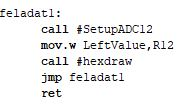
\includegraphics[scale=0.65]{1feladat}
\centering
\end{figure}

\section{AD átalakító kezelése II.}
A feladat az előzőhöz hasonlóan a potméter által beállított érték kiíratása volt, ezesetben azonban a jobb oldali potméter értékét kellett a jobb felső sarokba. Mivel a $hexdraw$ függvény csak a bal felső sarokba tud rajzolni, a korábbi mérésen már használt $LCDChrXY$ függvény hívásával rajzoltunk megfelelő koordinátákra. Jelen függvény azonban csak egy karakter kiírására alkalmas, így a beállított számot helyiértékenként kellett különböző koordinátákra kirajzolnunk, ezt a jobb oldalon található módszerrel oldottuk meg:


\begin{figure}[h]
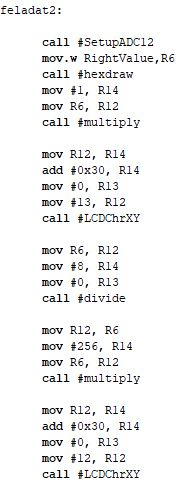
\includegraphics[scale=0.65]{2feladat_01}
\centering
\end{figure}


\begin{figure}[h]
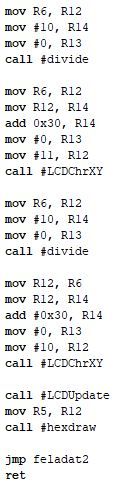
\includegraphics[scale=0.65]{2feladat_02}
\centering
\end{figure}

\section{Helyre történő kiíratás}
A feladat a korábbi méréshez hasonlóan a kijelző adott pontjába való kirajzolás, illetve a karakter mozgatása volt, ezesetben nem a joystick, hanem a két potméter segítségével. A bal oldali potméterrel az X, a jobb oldalival az Y koordináta értékét tudtuk módosítani. A feladat megvalósításához itt is az $LCDChrXY$ valamint az $LCDUpdate$ függvényeket használtuk a jobb oldali potméter értékét az R13, a bal oldaliét az R12 regiszterbe töltve, a kiírandó karakter kódját pedig az 'O' betűre állítva. Minden mozgatás után az előző karaktert kitöröltük egy 'space'-t írunk. 
A kódot a következő oldal tartalmazza. 




\section{Két ütő elkészítése}
A pong játékhoz tartozó két ütő elkészítése az előző feladathoz hasonlóan történt, a két potméter értékét beolvasva határoztuk meg a jobb illetve bal oldali ütő csak függőleges irányú elmozdulását, majd ugyancsak az $LCDChrXY$ függvény segítségével rajzoltuk ki a két ütőt alkotó egymás alatti két $0x23$ karakterkódú ütőt. 

\begin{figure}[h]
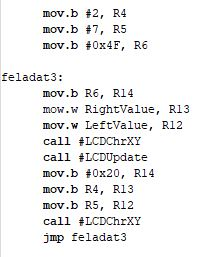
\includegraphics[scale=0.65]{3feladat}
\centering
\end{figure}

%Ha szeretnéd hogy az adott fejezet ne legyen számozva használj \section*{} -t, pl Acknowledgements


% Az egyenletekre, táblázatokra, listákra stb. itt nem térnék ki, ahhoz mindenképp érdemes kicsit utána olvasni

% A references mindig a legutolsó fejezet lesz

%  minden hivatkozás elnevezünk, ezzel a névvel fogunk hivatkozni a szövegen belül
% \bibitem{} <- hivatkozásnév
% A hivatkozás formája legjobban a példa dokumentumban látszik a tanárúr honlapján, általában: szerző, olvasott anyag neve, közreműködők, hely, év
% a szövegben pedig \cite{Megadott hivatkozásnév} -vel hivatkozunk


% példa:


% Ez a rész mindig marad:---------
\bibliographystyle{ieeetr}
%\bibliography{references}


% that's all folks
\end{document}
